\documentclass{scrartcl}



\usepackage{lmodern}
\usepackage[utf8]{inputenc}
\usepackage[T1]{fontenc}
\usepackage[onehalfspacing]{setspace}
\usepackage[stretch=10]{microtype}
\usepackage[english]{babel}

\usepackage[head=16.49677pt,top=32mm,bottom=32mm,left=25mm,right=25mm]{geometry}

\usepackage{xcolor}
\usepackage[pdftex]{graphicx}
\usepackage{float}
\usepackage{titling}
\usepackage{listings}
\usepackage{amsmath}
\usepackage{amsfonts}
\usepackage{booktabs}
\usepackage{multirow}
\usepackage{acronym}


\usepackage{xurl}
\usepackage{hyperref}



\usepackage{blindtext}

\usepackage[headsepline]{scrlayer-scrpage}
\automark{section}
\ihead{\headmark}
\chead{}
\ohead{\pagemark}
\ifoot{}
\cfoot{}
\ofoot{}


\usepackage[style=ieee]{biblatex}
\addbibresource{references/books.bib}
\addbibresource{references/papers.bib}
\addbibresource{references/online.bib}

\usepackage[toc, acronym]{glossaries}
% \makenoidxglossaries
% \loadglsentries{glossary.tex}


\newcommand{\ra}[1]{\renewcommand{\arraystretch}{#1}}

\usepackage{minted}
\usepackage{caption}
\usepackage{subcaption}
\usepackage{csquotes}
\usepackage{pgfplots}

\pgfplotsset{compat=1.17}
\pgfplotsset{every axis/.append style={tick label style={/pgf/number format/fixed},font=\scriptsize,ylabel near ticks,xlabel near ticks,grid=major}}


\setminted{xleftmargin=20pt,linenos,breaklines,fontsize=\footnotesize}
\setlength\parindent{0pt}
\definecolor{htwgruen}{RGB}{118, 185, 0}
\definecolor{htwblau}{RGB}{0, 130, 209}
\definecolor{htworange}{RGB}{255, 95, 0}
\definecolor{htwgrau}{RGB}{175, 175, 175}

\newcommand*{\gradeType}[1]{\gdef\thegradetype{#1}}
\newcommand*{\supervisor}[1]{\gdef\thesupervisor{#1}}
\newcommand*{\matrikelNo}[1]{\gdef\thematrikelno{#1}}
\newcommand*{\submitDate}[1]{\gdef\thesubmitdate{#1}}
\newcommand*{\university}[1]{\gdef\theuniversity{#1}}
\newcommand*{\department}[1]{\gdef\thedepartment{#1}}
\newcommand*{\email}[1]{\gdef\theemail{#1}}
\newcommand*{\class}[1]{\gdef\theclass{#1}}

\def\changemargin#1#2{\list{}{\rightmargin#2\leftmargin#1}\item[]}
\let\endchangemargin=\endlist

\renewcommand*{\maketitle}{
    \begin{titlepage}
        % Logo
        
        \begin{changemargin}{-0.8cm}{0.0cm}
            
\includegraphics[width=0.50\textwidth]{resources/images/Q01_HTW_Berlin_Logo_quer_pos_FARBIG_CMYK.eps}
        \end{changemargin}
        
    
        % Abstand nach logo
        \vspace{2.0cm}
    
        % Textkörper
        \begin{changemargin}{0.0cm}{0.0cm}
            % Dokumenttyp
            \color{htwgrau}
            \normalsize
            \textsf{\noindent\MakeUppercase{Title}} \vspace{-20pt}\\
            % Horizontale Linie
            \noindent\rule{\textwidth}{0.5pt}\vspace{-4pt}
            % Title
            \color{black}
            \huge
            \textsf{\thetitle}
            \vspace{12pt}
    
            % Author
            \color{htwgrau}
            \normalsize
            \textsf{AUTHOR}\\
            \color{black}
            \large
            \textsf{\theauthor}
            
            % E-Mail
            \color{htwgrau}
            \normalsize
            \textsf{E-MAIL}\\
            \color{black}
            \large
            \textsf{\theemail{}}
    
    
            % Am Ende der Seite
            \vfill

            % University
            \color{htwgrau}
            \normalsize
            \textsf{CLASS}\\
            \color{black}
            \large
            \textsf{\theclass}
    
            % University
            \color{htwgrau}
            \normalsize
            \textsf{UNIVERSITY}\\
            \color{black}
            \large
            \textsf{\theuniversity}
            
            % University
            \color{htwgrau}
            \normalsize
            \textsf{DEPARTMENT}\\
            \color{black}
            \large
            \textsf{\thedepartment}
    
            % Supervisor
            \color{htwgrau}
            \normalsize
            \textsf{SUPERVISOR}\\
            \color{black}
            \large
            \textsf{\thesupervisor}
        \end{changemargin}
        


    \end{titlepage}
}


\title{Implementation of a GAN-architecture}
\author{Christoph Stach}
\matrikelNo{0555912}
\university{Hochschule für Technik und Wirtschaft Berlin}
\department{Fachbereich 4 - Angewandte Informatik}
\email{s0555912@htw-berlin.de}
\class{Independent Coursework 1}

\supervisor{Prof. Dr. Christian Herta\\Patrick Baumann}


\begin{document}


\maketitle

\newpage

\begin{abstract}
    \thispagestyle{empty}
    \begin{changemargin}{2.0cm}{2.0cm}
        
        \vspace*{\fill}
        \begin{center}
            \Large
            \textbf{Abstract}
            \vspace{0.5cm}
        \end{center}

        \large
        This project demonstrates the usage of Generative Adversarial Networks to generate new images of a given domain. The author uses an often used network architecture combined with a successfully proven loss function to train multiple models. He demonstrates the flexibility of this approach by using networks of different depths. Training is performed on two image datasets, and the results are presented at the end of the document. The chosen approach can generate RGB images, which look similar to the source dataset, but usually contain generation artifacts. 

        \vspace*{\fill}
    \end{changemargin}
\end{abstract}

\newpage

\pagenumbering{roman}


% \addcontentsline{toc}{section}{Contents}
\thispagestyle{empty}
\tableofcontents


\newpage
\thispagestyle{empty}
\addcontentsline{toc}{section}{\listfigurename}

\listoffigures
\addcontentsline{toc}{section}{\listtablename}
\listoftables

\addcontentsline{toc}{section}{\lstlistlistingname}
\lstlistoflistings


\newpage


\pagenumbering{arabic}

\section{Introduction}

Computer science's independent coursework project will be about image generation with Generative Adversarial Networks (GAN). The goal is to examine GANs and explore their capability of generating new images of arbitrary datasets. This project uses photorealistic paintings, but the proposed application can also create a different format. Generative Adversarial Networks is a research area of deep learning, where two (or more) Neural Networks are competing. In a standard GAN architecture, a Generator creates images from a random number vector. A Discriminator decides if the image comes from the Generator or the actual dataset. The Generator continuously tries to fool the Discriminator and therefore creates images of increasing quality.


\subsection{Motivation}

Early GAN implementations used Dense-layers to generate new data. Follow-up projects like DCGAN used Convolutional-layers, which are better suited for computer vision and image tasks. Still, it was tough to train networks with the capability of generating larger images. Training often was unstable and suffered from problems like Mode-Collapse. GANs require datasets of vast size and sufficient computing power. These reasons make GANs an exciting research topic.

\subsection{Objective}

The project aims to develop a GAN-model capable of creating new images from a given dataset. The focus lies on generating images of faces. It should create images in RGB-format bigger than the ones from the traditional MNIST-dataset (28x28 pixels), at least 64x64 pixels. The developed pipeline should be flexible to create models of different sizes. The training progress should converge and avoid failure modes like Mode-Collapse. Creating a GAN framework that satisfies the mentioned requirements and is stable to train is the goal. That includes finding an appropriate model architecture, loss function, optimizer, and hyperparameter configuration. 


\subsection{Constrains}

As GANs need a lot of computing power and time to train, this project only generates images of a maximum size of 64x64 pixels, due to limited computing resources. The requirement is that the GAN architecture is implemented in PyTorch and trained with the Determined AI framework. \newpage
\section{Fundamentals}

In the section fundamentals, the author explains the necessary theoretical techniques to understand the Generative Adversarial Network framework. The author references essential literature in the GAN research area and introduces the general GAN framework, a often used network architecture, and an improved loss function to train GANs.

\subsection{Generative Adversarial Network}

\citeauthor{goodfellow2014generative} first introduced GANs \cite{goodfellow2014generative}. They created a framework of two Neural Networks which are co-trained. One they call the Generator, it takes a random noise vector as an input and transforms it to generate data in the form of images. The other one they call the Discriminator, which decides if the image is fake or not. It takes data in the form of images and tries to estimate if the given image comes from a real dataset, in their case, the MNIST dataset or from the Generator.\\

In other words the Generator transforms the noise distribution $ p_{z}(z) $ to $ p_{g} $. The learning process then tries to shift $ p_{g} $ towards the real data distribution $ p_{data} $. So that under optimal conditions the $ p_{g} $ and $  p_{data} $ are indistinguishable by the Discriminator.\\

\begin{figure}[H]
    \centering
    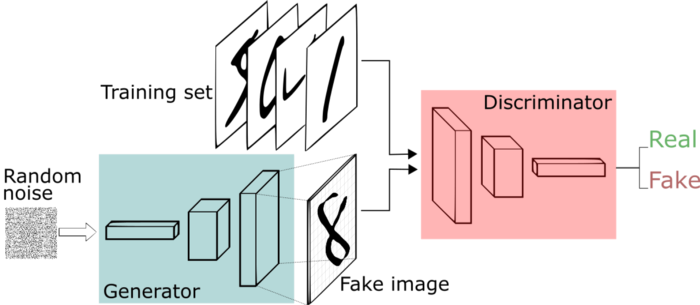
\includegraphics[width=0.65\textwidth]{resources/images/gan.png}
    \caption{Illustration of the general architecture of a Generative Adverserial Network. By \citeauthor{twd:gan} \cite{twd:gan}.}
    \label{fig:gan}
\end{figure}

They use the following training objective in the form of a value function. Their implementation negates the formula to create the corresponding loss function.\\

\begin{equation}
    \min _{G} \max _{D} V(D, G)=\mathbb{E}_{\boldsymbol{x} \sim p_{\text {data }}(\boldsymbol{x})}[\log D(\boldsymbol{x})]+\mathbb{E}_{\boldsymbol{z} \sim p_{\boldsymbol{z}}(\boldsymbol{z})}[\log (1-D(G(\boldsymbol{z})))]
\end{equation}\\

\newpage

To train the GAN, they update the Discriminator more often than the Generator. For each iteration, they alter the Discriminator weights $ k $ times and perform gradient ascend based on the following loss function:\\
unseen images
\begin{equation}
    \nabla_{\theta_{d}} \frac{1}{m} \sum_{i=1}^{m}\left[\log D\left(\boldsymbol{x}^{(i)}\right)+\log \left(1-D\left(G\left(\boldsymbol{z}^{(i)}\right)\right)\right)\right]
\end{equation}\\

Afterward, the Generator is updated once with gradient ascend and the loss function:\\

\begin{equation}
    \nabla_{\theta_{g}} \frac{1}{m} \sum_{i=1}^{m} \log \left(1-D\left(G\left(\boldsymbol{z}^{(i)}\right)\right)\right)
\end{equation}\\

\subsection{Deep Convolutional GAN}

Deep Convolutional GAN (DCGAN) is an advancement of the original GAN model proposed by \citeauthor{goodfellow2014generative}.  \citeauthor{radford2016dcgan} developed it in 2015. Compared to GAN, it uses purely convolutional operations instead of the used Dense-layers in the first GAN architecture.\\

\begin{figure}[H]
    \centering
    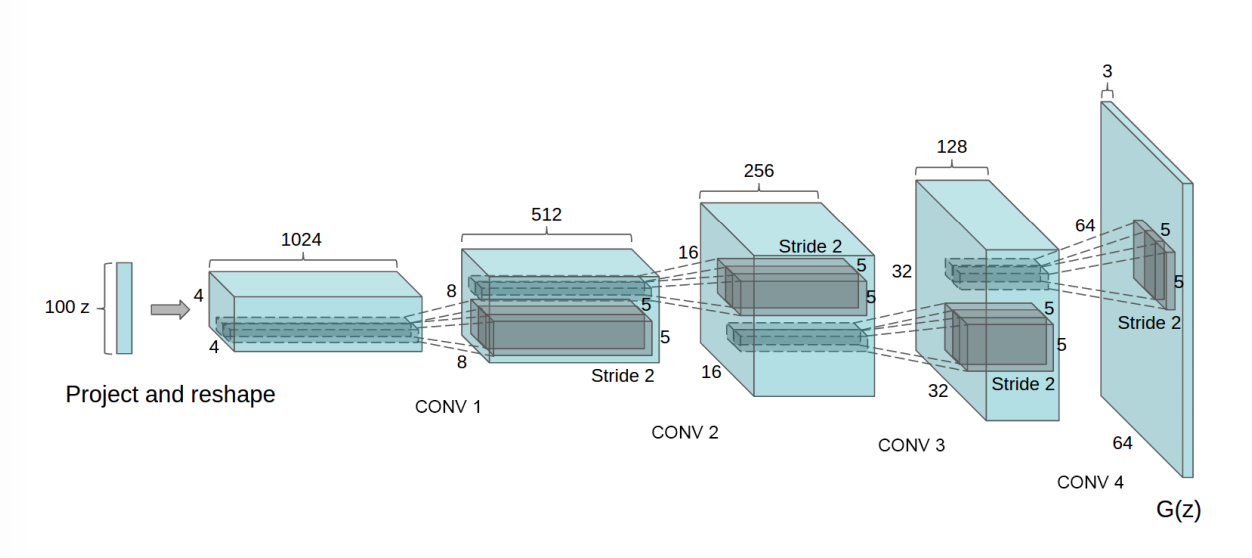
\includegraphics[width=0.65\textwidth]{resources/images/dcgan_generator.png}
    \caption{The Generator architecture proposed by \citeauthor{radford2016dcgan} in \citetitle{radford2016dcgan} \cite{radford2016dcgan}.}
    \label{fig:dcgan_generator}
\end{figure}

\citeauthor{radford2016dcgan} develop the following guidelines for the GAN architecture based on convolutional layers.

\begin{itemize}
    \item Replace any pooling layers with strided convolutions (Discriminator) and fractional-strided convolutions (Generator).
    \item Use batch-normalization in both the Generator and the Discriminator.
    \item Remove fully connected hidden layers for deeper architectures.
    \item Use ReLU activation in Generator for all layers except for the output, which uses Tanh.
    \item Use LeakyReLU activation in the Discriminator for all layers.
\end{itemize}


They claim by applying these guidelines they could improve the stability of the adversarial training. They also identify that sometimes the models collapse to a subset or a single mode if training time was too long.\\

Today's more modern GAN implementations often use DCGAN as a baseline and build their architecture upon the original one. Often the proposed guidelines are partially applied.\\

\subsection{Wasserstein GAN}

\citeauthor{arjovsky2017wgan} proposed Wasserstein GAN (WGAN) in 2017. It uses a new loss function that stabilizes the training. Before the success of WGAN, GANs commonly used loss functions that approximate the Kullback-Liber divergence or the Jensen–Shannon divergence. These divergences measure the distance between two data distributions. In GANs, the generated and the actual data distribution. WGAN proposes to use Earthmover's Distance instead. Their implementation removes the final Sigmoid-Activation from the Discriminator to allow the output to be unbound. Also, they perform weight-clipping after each gradient step to ensure the function is Lipschitz-1.\\


\begin{figure}[H]
    \centering
    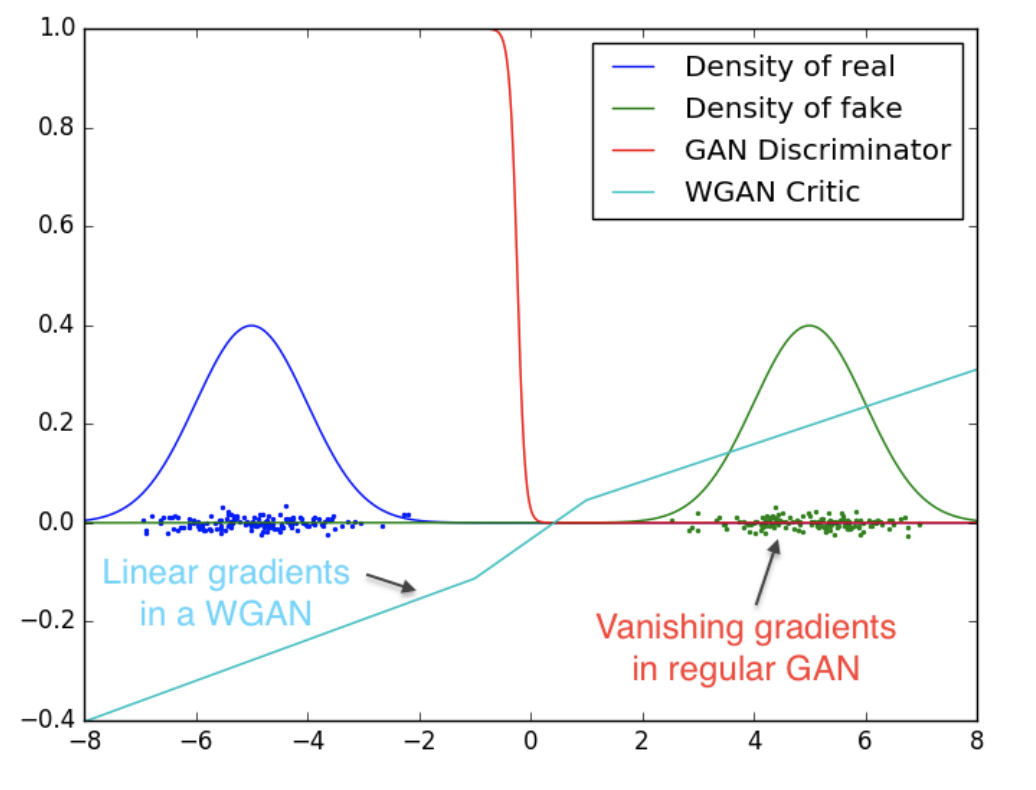
\includegraphics[width=0.65\textwidth]{resources/images/wgan1.png}
    \caption{The picture shows how WGAN performs compared to traditional GAN. WGAN can deliver strong gradients even if the two distributions do not overlap. The gradient signal vanishes for GANs.}
    \label{fig:wgan1}
\end{figure}

 
\subsubsection{Earthmover's Distance}

The Earthmover's Distance (EMD) \cite{emd} measures the work necessary to move the earth between two landmasses to make them equal. The following formula defines the EMD or Wasserstein-1 for two data distributions $ \mathbb{P}_{r} $  and $ \mathbb{P}_{g} $.\\

\begin{equation}
    W\left(\mathbb{P}_{r}, \mathbb{P}_{g}\right)=\inf _{\gamma \in \Pi\left(\mathbb{P}_{r}, \mathbb{P}_{g}\right)} \mathbb{E}_{(x, y) \sim \gamma}[\|x-y\|]
\end{equation}\\

The WGAN loss function approximates the EMD for the actual data distribution $ \mathbb{P}_{g} $ and a parameterized data distribution $ \mathbb{P}_{\theta} $. The condition is that the Discriminator $ f $ is Lipschitz-1.\\

\begin{equation}
    W\left(\mathbb{P}_{r}, \mathbb{P}_{\theta}\right)=\sup _{\|f\|_{L} \leq 1} \mathbb{E}_{x \sim \mathbb{P}_{r}}[f(x)]-\mathbb{E}_{x \sim \mathbb{P}_{\theta}}[f(x)]
\end{equation}\\

\subsubsection{Lipschitz Continuity}

The WGAN loss requires a Discriminator that is Lipschitz-1 constrained. The Lipschitz Continuity \cite{Eriksson2004lipschitz} describes the functions property how fast it can change.  A Lipschitz-continues function with a Lipschitz constant $ L_{f}=1 $ has the property that it continues at any point within a given interval $ I $. Further, it can only change by a maximum absolute value of 1 between two consecutive steps. That means that the absolute derivate at any point of the function is never higher than 1. Such a function is called Lipschitz-1.\\

\begin{equation}
    \left|f\left(x_{1}\right)-f\left(x_{2}\right)\right| \leq L_{f}\left|x_{1}-x_{2}\right| \quad \text { for all } x_{1}, x_{2} \in I
\end{equation}\\

A small Lipschitz constant $ L_{f} $ signifies that small changes in the function's input parameters yield small changes in its output. On the other hand, a high value for  $ L_{f} $ means that small changes in the input parameters can significantly affect the function's output.\\

In their work, they clip the Discriminator's weights by the factor $ c $ to enforce the Lipschitz constraint. They state that it is a terrible way to ensure the property and that the training's performance is sensitive to the choice of $ c $.

\subsubsection{Gradient Penalty}

For the reasons metioned above \citetitle{gulrajani2017wgangp} \cite{gulrajani2017wgangp} \citeauthor{gulrajani2017wgangp} demonstrate how an additional loss regularization term can replace the weight-clipping technique. They introduce a gradient penalty that does not suffer from the same weaknesses as weight-clipping.\\

\begin{equation}
    \lambda \underset{\hat{x} \sim \mathbb{P}_{\hat{x}}}{\mathbb{E}}\left[\left(\left\|\nabla_{\hat{\boldsymbol{x}}} f(\hat{\boldsymbol{x}})\right\|_{2}-1\right)^{2}\right]
\end{equation}\\

The equation above regularizes the Discriminator to have gradients with the norm of 1 almost everywhere. The gradient penalty randomly samples  $ x $ from $ \mathbb{P}_{\hat{x}} $ where $ \mathbb{P}_{\hat{x}} $ are the straight lines between $ \mathbb{P}_{g} $ and $ \mathbb{P}_{r} $. \newpage
\section{Methodology}

The section methodology describes the techniques, software, and datasets used to realize the project. Furthermore, the author gives insight into concrete implementation details.

\subsection{Technologies}

The development of a GAN is possible with various technologies. This section briefly introduces the core technologies of the project.

\subsubsection{PyTorch}

PyTorch\footnote{PyTorch: \url{https://pytorch.org/}} is an open-source machine learning framework developed by Facebook. It provides automatic differentiation of arbitrary composed functions and is widely used to develop neural network architectures.

\subsubsection{Determined AI}

Determined AI\footnote{Determined AI: \url{https://determined.ai/}} is a self-hosted open-source deep learning platform. It helps set up a distributed model training environment and supports various deep learning frameworks, including PyTorch. It allows developers to train models on multiple machines and also supports hyperparameter search.

\subsection{Datasets}

GANs require a large amount of data to train. The author uses two different datasets to test the implementation of the architecture.

\subsubsection{CelebA HQ}

The CelebA HQ dataset is a post-processed version of the CelebA\footnote{CelebA: \url{http://mmlab.ie.cuhk.edu.hk/projects/CelebA.html}} dataset \cite{liu2015faceattributes}. \citeauthor{karras2018progressive} introduced it in \citetitle{karras2018progressive} \cite{karras2018progressive}, and it consists of 30.000 high definition images of celebrity faces.


\subsubsection{Anime Face}

The Anime Face\footnote{Anime Face: \url{https://github.com/bchao1/Anime-Face-Dataset}} is a large dataset consisting of low-definition images ($ \sim 90*90 - 120*120 $). After the deletion of corrupted files, it has 63.632 files in total.


\subsection{Implementation}

By presenting concrete source code examples, the author explains the essential parts of the project. The complete source code is available under \url{https://github.com/christophstach/htw-icw1-implementation}.

\subsubsection{Model Architecture - Generator}

The following table describes the Network architecture of the Generator. The input variable flows through multiple transposed convolutions followed by the non-linearity ReLU and a batch normalization operation \cite{ioffe2015batchnorm}. The transposed convolution is responsible for scaling the tensor's width and height up by a factor of two and reducing the channel dimension at the same time. The last layer transforms the tensor to an RGB-Image using a Tanh activation and omitting the batch norm operation. \\


Kernel size = $ K $,
Stride = $ S $,
Padding = $ P $,
Activation = $ \sigma $,
Normalization = $ N $ \\

\begin{table}[H]
    \ra{1.3}
    \centering
    \begin{tabular}{@{}llllllll@{}}
        \toprule
        Operation              & In              & Out              & $ K $ & $ S $ & $ P $ & $ \sigma $ & $ N $ \\ \midrule
        Transposed Convolution & $ 128 * 1 * 1 $ & $ 8 * 4 * 4 $    & $ 4 $ & $ 1 $ & $ 1 $ & ReLU       & Batch \\
        Transposed Convolution & $ 8 * 4 * 4 $   & $ 4 * 8 * 8 $    & $ 4 $ & $ 2 $ & $ 1 $ & ReLU       & Batch \\
        Transposed Convolution & $ 4 * 8 * 8 $   & $ 2 * 16 * 16 $  & $ 4 $ & $ 2 $ & $ 1 $ & ReLU       & Batch \\
        Transposed Convolution & $ 2 * 16 * 16 $ & $ 1 * 32 * 32 $  & $ 4 $ & $ 2 $ & $ 1 $ & ReLU       & Batch \\
        Transposed Convolution & $ 1 * 32 * 32 $ & $ 3 * 64 * 64 $  & $ 4 $ & $ 2 $ & $ 1 $ & Tanh       & -     \\ \bottomrule
    \end{tabular}
    \caption{Network architecture of the Generator}
    \label{tab:architecture-generator}
\end{table}

The first dimension of In and Out is the channel dimension. The author multiplies the channel dimension with an additional factor $ G_{Depth} $ to scale the network. The \autoref{sec:evaluation} \nameref{sec:evaluation} conducts multiple experiments with different network sizes. \\



\newpage

\subsubsection{Model Architecture - Discriminator}

The Discriminator's architecture reverses the Generator's one. It accepts an RGB-Image of the size $ 3* 64 * 64 $ as input. The image flows through multiple convolutional layers of which each has a stride of two, which results in a downsampling effect. This results in a halved width and height but a doubled number of channels. \\

\begin{table}[H]
    \ra{1.3}
    \centering
    \begin{tabular}{@{}llllllll@{}}
        \toprule
        Operation   & In              & Out              & $ K $ & $ S $ & $ P $ & $ \sigma $ & $ N $ \\ \midrule
        Convolution & $ 3 * 64 * 64 $ & $ 1 * 32 * 32 $  & $ 4 $ & $ 2 $ & $ 1 $ & LReLU(0.2) & Layer \\
        Convolution & $ 1 * 32 * 32 $ & $ 2 * 16 * 16 $  & $ 4 $ & $ 2 $ & $ 1 $ & LReLU(0.2) & Layer \\
        Convolution & $ 2 * 16 * 16 $ & $ 4 * 8 * 8   $  & $ 4 $ & $ 2 $ & $ 1 $ & LReLU(0.2) & Layer \\
        Convolution & $ 4 * 8 * 8 $   & $ 8 * 4 * 4   $  & $ 4 $ & $ 2 $ & $ 1 $ & LReLU(0.2) & Layer \\
        Convolution & $ 8 * 4 * 4 $   & $ 1 * 1 * 1   $  & $ 4 $ & $ 1 $ & $ 0 $ & -          & -     \\ \bottomrule
    \end{tabular}
    \caption{Network architecture of the Discriminator}
    \label{tab:architecture-discriminator}
\end{table}

The Discriminator uses the leaky ReLU activation function,  width a negative slope of 0.2, followed by a layer normalization \cite{ba2016layernorm} operation after each convolution. In the end, the network outputs a value that represents a score and can be used to calculate the Earth mover's distance. Compared to the standard GAN \cite{goodfellow2014generative}, WGAN \cite{arjovsky2017wgan} omits the last sigmoid function, which calculates an image's probability from the actual data distribution. WGAN requires an unbound value to calculate the loss. \\


\begin{figure}[H]
    \centering
    \begin{subfigure}[b]{0.3\textwidth}
        \centering
        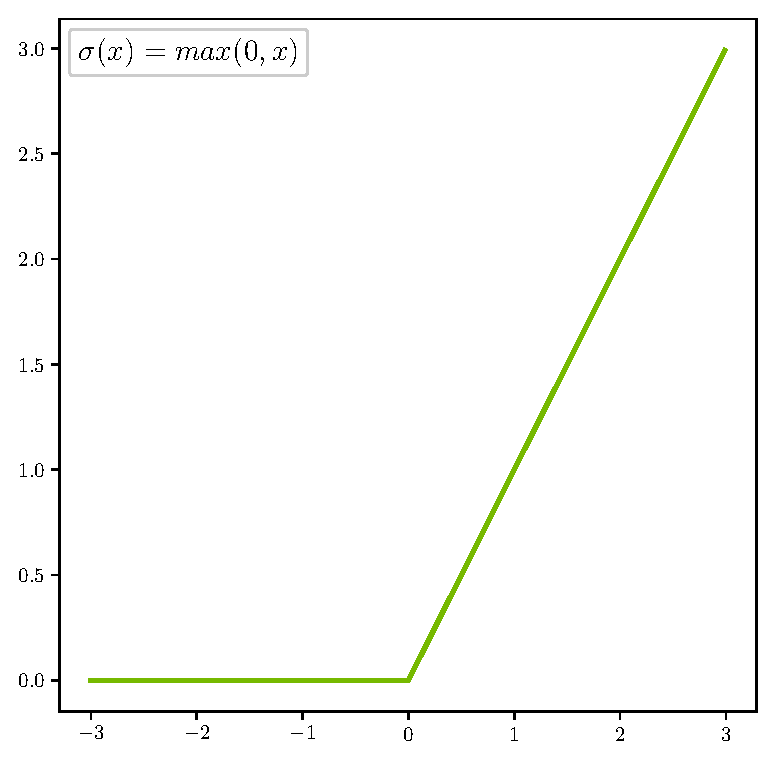
\includegraphics[width=\textwidth]{resources/images/ReLU.eps}
        \caption{ReLU\footnotemark}
        \label{fig:relu}
    \end{subfigure}
    \hfill
    \begin{subfigure}[b]{0.3\textwidth}
        \centering
        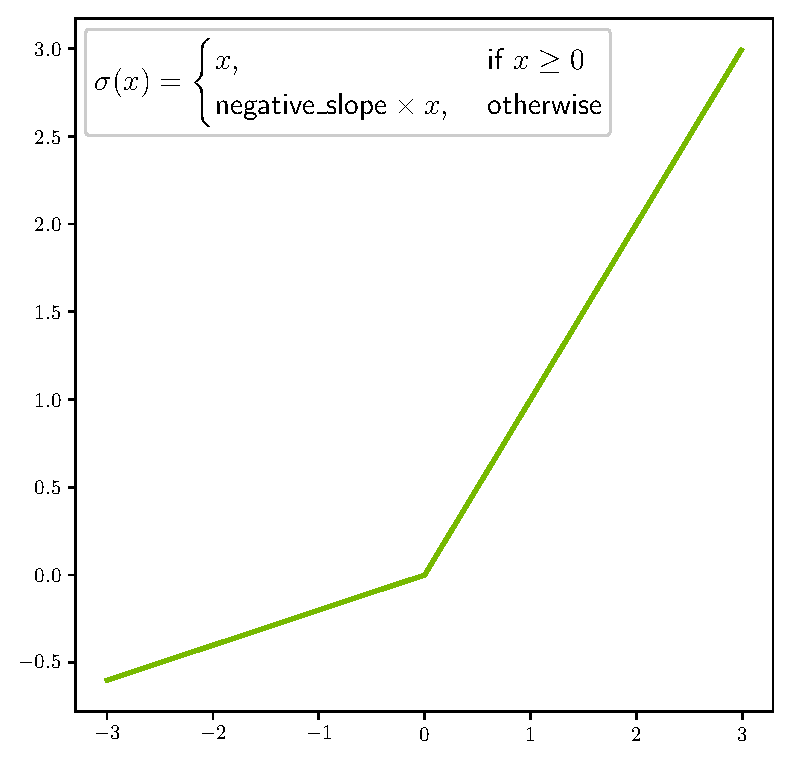
\includegraphics[width=\textwidth]{resources/images/LReLU.eps}
        \caption{LReLU\footnotemark}
        \label{fig:lrelu}
    \end{subfigure}
    \hfill
    \begin{subfigure}[b]{0.3\textwidth}
        \centering
        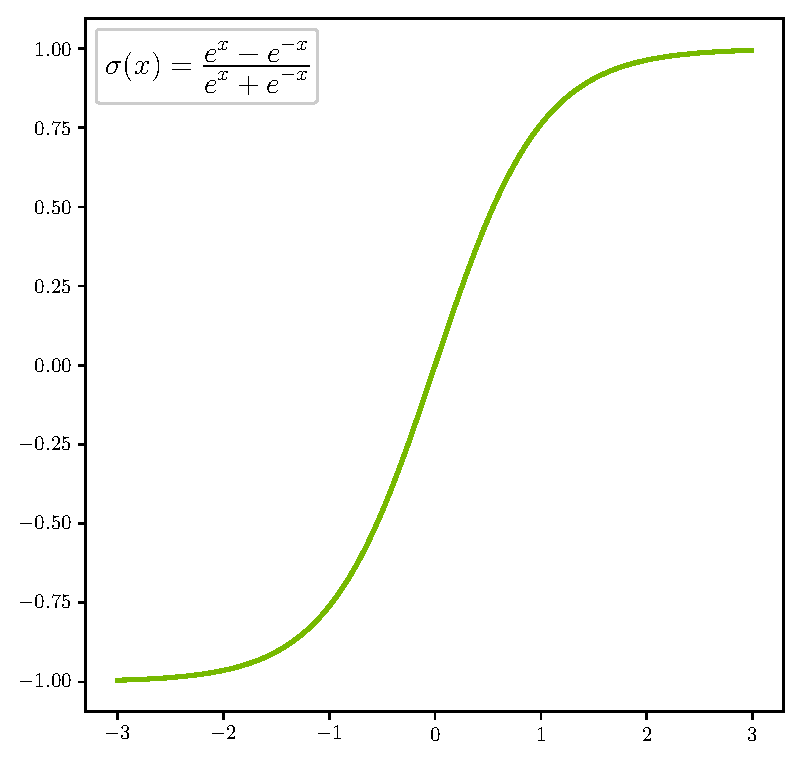
\includegraphics[width=\textwidth]{resources/images/Tanh.eps}
        \caption{Tanh\footnotemark}
        \label{fig:tanh}
    \end{subfigure}
    \caption{The Generator and Discriminator use these 3 activation functions: ReLU, LReLU and Tanh}
    \label{fig:activation_functions}
\end{figure}


\footnotetext[5]{ReLU: \url{https://pytorch.org/docs/stable/generated/torch.nn.ReLU.html}}
\footnotetext[6]{LReLU: \url{https://pytorch.org/docs/stable/generated/torch.nn.LeakyReLU.html}}
\footnotetext[7]{Tanh: \url{https://pytorch.org/docs/stable/generated/torch.nn.Tanh.html}}


\newpage


\subsubsection{Determined AI - Training Loop}

The Determined AI training loop is a simple method of the PyTorchTrial class. Determined AI passes batches from the configured data loader of the configured batch size to this method. The function is responsible for optimizing the neural networks. The user can decide which values he wants to return and make available on the Determined AI dashboard. In the case of this project, the author returns multiple different loss values. \\

\begin{listing}[H]
\inputminted{python}{resources/codes/train_batch.py}
\captionof{lstlisting}{The main training loop method of Determined AI}
\end{listing}

The first step in a WGAN is to optimize the Discriminator. To do that, one needs to sample a  random vector $ z $ from a normal distribution and pass it to the Generator to create fake images. Fake images and actual images pass through the Discriminator and their scores through the loss function and the gradient penalty function, which the author explains in \ref{sec:loss_function} and \ref{sec:gradient_penalty}. The total loss is the sum of the two. Determined AI offers methods to calculate the backward pass and perform the optimization step. Note that in lines 5-6, the Generator gradients are not calculated.  \\

\begin{listing}[H]
\inputminted{python}{resources/codes/optimize_discriminator.py}
\captionof{lstlisting}{How to opimize the Discriminator}
\end{listing}

\newpage

To train the Generator, the Discriminator only needs to calculate the scores of the generated fake images. The scores pass to the Generator's loss function, and the backward function uses the loss to calculate the gradients. Afterward, the Generator's optimizer performs an optimization step on the Generator's weights.

\begin{listing}[H]
\inputminted{python}{resources/codes/optimize_generator.py}
\captionof{lstlisting}{How to opimize the Generator}
\end{listing}

\subsubsection{Loss Function}
\label{sec:loss_function}

Generator and Discriminator use different loss functions. Both loss functions together form the WGAN loss. Adding the negative mean of the actual images' scores and the positive mean of the fake images' scores calculates the Discriminator loss. The Generator's loss calculates by averaging over the negative scores of the fake images.

\begin{listing}[H]
\inputminted{python}{resources/codes/wgan_loss.py}
\captionof{lstlisting}{Code for the WGAN-Loss}
\end{listing}


\newpage

\subsubsection{Gradient Penalty}
\label{sec:gradient_penalty}

Adding a regularization term to the Discriminator's total loss ensures that the Discriminator satisfies the  Lipschitz-1 constraint.

\begin{listing}[H]
\inputminted{python}{resources/codes/gradient_penalty.py}
\captionof{lstlisting}{Code of the Gradient Penalty}
\end{listing}

Line 1-2 calculate an intermediate image representation by picking a random location on a straight line between real and fake images. These interpolated images pass to the Discriminator in Line 5. Afterward, PyTorch's autograd calculates the Discriminator's gradients. Line 9 forms the Euclidean norm of each tensor in the gradients batch, then subtracts it by one and takes it to the power of two. The final gradient penalty is the mean of the before calculated norms multiplied with a coefficient of 10.

\newpage

\subsection{Evaluation}
\label{sec:evaluation}


The author performs eight different experiments to test the performance and the image quality of the generated images. All experiments use Adam as the optimizer for Discriminator and Generator. The author sets the Discriminators learning rate to $ 0.0004 $ and the Generators learning rate to $ 0.0001 $. This configuration is in the paper \citetitle{heusel2018ttur} \cite{heusel2018ttur}. It proves that it can omit the need for multiple Discriminator updates. \\


\begin{table}[H]
    \ra{1.3}
    \centering
    \begin{tabular}{@{}lllllllll@{}}
    \toprule
    \# & Optimizer & $ lr_{g} $ & $ lr_{d} $ & $ \beta_{g} $ & $ \beta_{d} $ & $ depth_{g} $ & $ depth_{d} $ & $ dim_{z} $ \\ \midrule
    1 & Adam & 0.0001 & 0.0004 & 0.5, 0.999 & 0.5, 0.999 & 8  & 8  & 128 \\
    2 & Adam & 0.0001 & 0.0004 & 0.5, 0.999 & 0.5, 0.999 & 16 & 16 & 128 \\
    3 & Adam & 0.0001 & 0.0004 & 0.5, 0.999 & 0.5, 0.999 & 32 & 32 & 128 \\
    4 & Adam & 0.0001 & 0.0004 & 0.5, 0.999 & 0.5, 0.999 & 64 & 64 & 128 \\ \bottomrule
    \end{tabular}
    \caption{Experiment configurations with the CelebA HQ dataset}
\label{tab:experiments_celeba_hq}
\end{table}

Both optimizers use the same beta values $ \beta_{1} $ and $ \beta_{2} $ of 0.5 and 0.999. All experiments transform the vector $ z $ with a dimension of 128 to 64x64 RGB images. Each experiment varies in the Generators and Discriminator's depth. The depth is a multiplier for the number of filters in the networks. A higher depth means more parameters and, therefore more trainable degree of freedom. The experiments examine the effect of the depth parameter on the generated image quality. \\

\begin{table}[H]
    \ra{1.3}
    \centering
    \begin{tabular}{@{}lllllllll@{}}
    \toprule
    \# & Optimizer & $ lr_{g} $ & $ lr_{d} $ & $ \beta_{g} $ & $ \beta_{d} $ & $ depth_{g} $ & $ depth_{d} $ & $ dim_{z} $ \\ \midrule
    5 & Adam & 0.0001 & 0.0004 & 0.5, 0.999 & 0.5, 0.999 & 8  & 8  & 128 \\
    6 & Adam & 0.0001 & 0.0004 & 0.5, 0.999 & 0.5, 0.999 & 16 & 16 & 128 \\
    7 & Adam & 0.0001 & 0.0004 & 0.5, 0.999 & 0.5, 0.999 & 32 & 32 & 128 \\
    8 & Adam & 0.0001 & 0.0004 & 0.5, 0.999 & 0.5, 0.999 & 64 & 64 & 128 \\ \bottomrule
    \end{tabular}
    \caption{Experiment configurations with the Anime Face dataset}
\label{tab:experiments_anime_face}
\end{table}

\newpage \newpage

\section{Results}

In the results section, the author describes his observations on the different models defined in section 3.4. The training used a batch size of 64. In total, each model was trained over 500.000 batches. \\

\begin{figure}[H]
    \centering
    \begin{subfigure}[b]{0.45\textwidth}
        \centering
        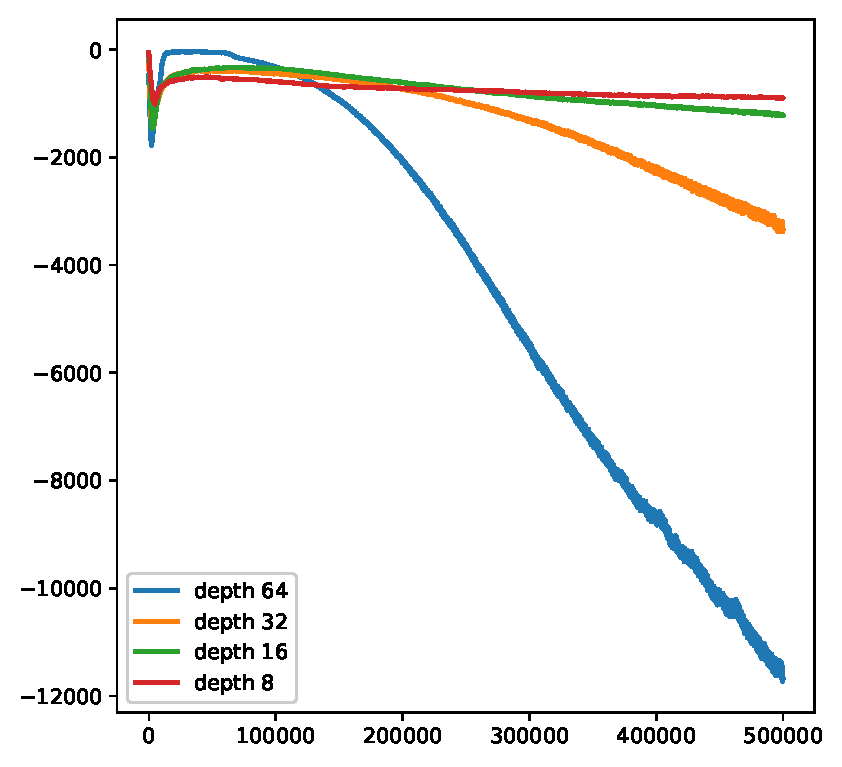
\includegraphics[width=\textwidth]{resources/images/celeba_hq_d_loss.eps}
        \caption{Anime Face}
        \label{fig:celeba_hq_d_loss}
    \end{subfigure}
    \hfill
    \begin{subfigure}[b]{0.45\textwidth}
        \centering
        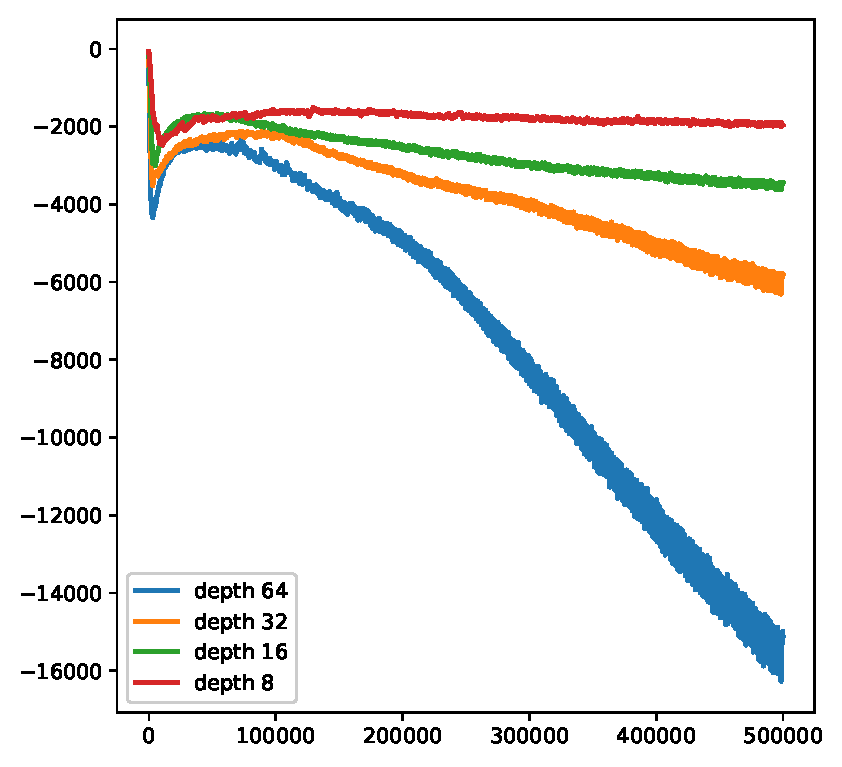
\includegraphics[width=\textwidth]{resources/images/anime_face_d_loss.eps}
        \caption{CelebA HQ}
        \label{fig:anime_face_d_loss}
    \end{subfigure}
    \caption{Discriminator loss curves}
    \label{fig:d_loss}
\end{figure}

The graphic above shows the loss curves of different models. One can see that with a higher model depth (which means more model parameters), the discriminator loss falls faster. That confirms the observations of the authors of \cite{arjovsky2017wgan}. They note that the discriminator loss correlates with the image quality. Therefore it makes sense that networks with more parameters can generate better-looking images. \\

\begin{figure}[H]
    \centering
    \begin{subfigure}[b]{0.24\textwidth}
        \centering
        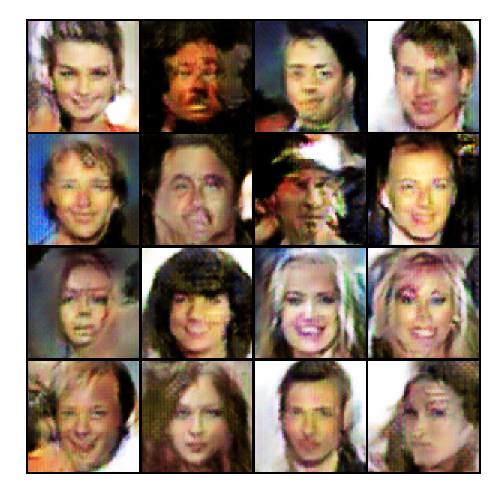
\includegraphics[width=\textwidth]{resources/images/output_celeba_8.eps}
        \caption{depth 8}
        \label{fig:celeba_8}
    \end{subfigure}
    \hfill
    \begin{subfigure}[b]{0.24\textwidth}
        \centering
        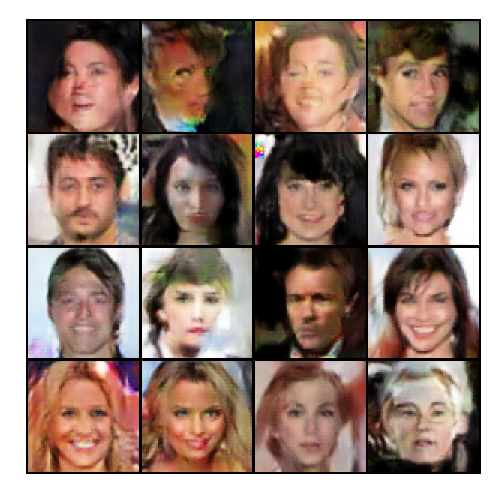
\includegraphics[width=\textwidth]{resources/images/output_celeba_16.eps}
        \caption{depth 16}
        \label{fig:celeba_16}
    \end{subfigure}
    \hfill
    \begin{subfigure}[b]{0.24\textwidth}
        \centering
        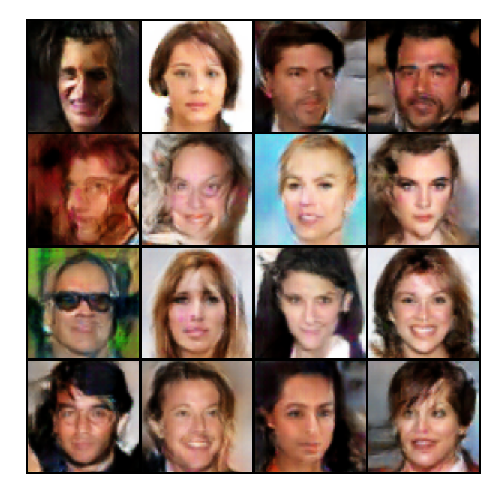
\includegraphics[width=\textwidth]{resources/images/output_celeba_32.eps}
        \caption{depth 32}
        \label{fig:celeba_32}
    \end{subfigure}
    \hfill
    \begin{subfigure}[b]{0.24\textwidth}
        \centering
        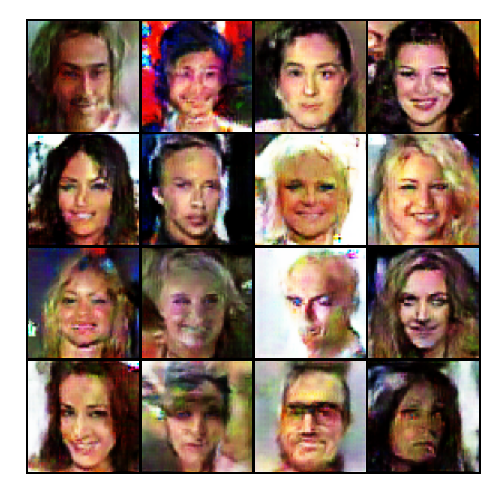
\includegraphics[width=\textwidth]{resources/images/output_celeba_64.eps}
        \caption{depth 64}
        \label{fig:celeba_64}
    \end{subfigure}
    \caption{Sample generated images of different models trained on the Celeba HQ dataset}
    \label{fig:output_celeba}
\end{figure}

The graphic above shows sample images generated by the networks trained on the Celeba HQ dataset. It is clear to see that the networks with smaller depth produce less appealing photos. The images generated by the depth 8 network do clearly show many artifacts. In this experiment, the depth 32 network delivers the best results. Some of the generated pictures look almost like human faces. Others have artifacts but less than the pictures generated by the networks with a lower depth. Also, this network learned about face accessories, as one person is wearing glasses on the image. The depth 64 network produces images with many artifacts. A possible reason is that the training process ran into a local minimum, which it couldn't escape from anymore. Another explanation is that a network with a depth of 64 is overparameterized, and the training process needs more time to converge.

\begin{figure}[H]
    \centering
    \begin{subfigure}[b]{0.24\textwidth}
        \centering
        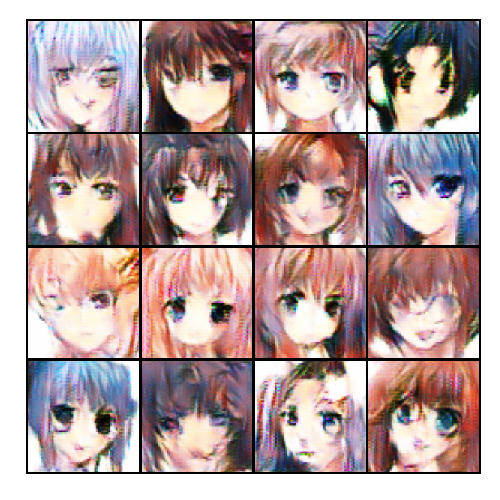
\includegraphics[width=\textwidth]{resources/images/output_anime_8.eps}
        \caption{depth 8}
        \label{fig:anime_8}
    \end{subfigure}
    \hfill
    \begin{subfigure}[b]{0.24\textwidth}
        \centering
        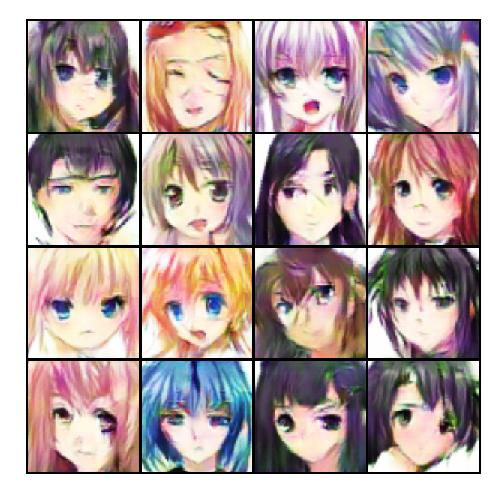
\includegraphics[width=\textwidth]{resources/images/output_anime_16.eps}
        \caption{depth 16}
        \label{fig:anime_16}
    \end{subfigure}
    \hfill
    \begin{subfigure}[b]{0.24\textwidth}
        \centering
        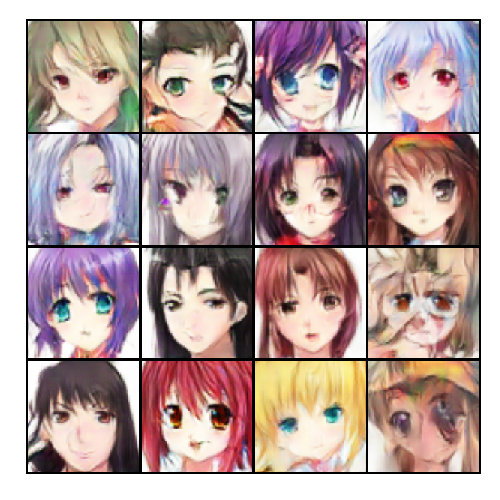
\includegraphics[width=\textwidth]{resources/images/output_anime_32.eps}
        \caption{depth 32}
        \label{fig:anime_32}
    \end{subfigure}
    \hfill
    \begin{subfigure}[b]{0.24\textwidth}
        \centering
        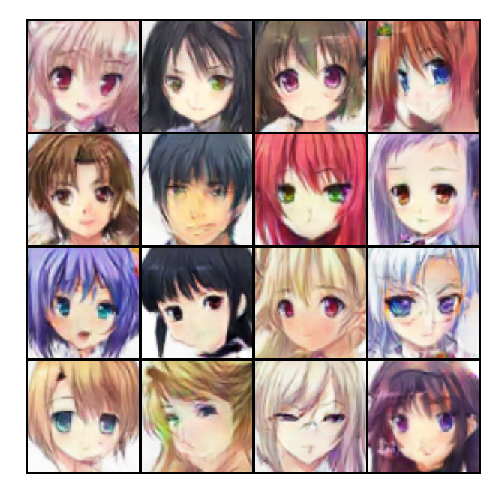
\includegraphics[width=\textwidth]{resources/images/output_anime_64.eps}
        \caption{depth 64}
        \label{fig:anime_64}
    \end{subfigure}
    \caption{Sample generated images of different models trained on the Anime Face dataset}
    \label{fig:ouput_anime}
\end{figure}

Similar observations can be made by looking at the generated pictures of the network trained on the Anime Face dataset. The networks with lower depth produce more artifacts. Also, the variety of the generated images is lower than in images generated by the higher parameterized networks. It is important to note that the depth 64 network, in this case, delivers excellent results. Most pictures look very similar to the images in the real Anime Face dataset. 

\subsection{Conclusion}

In this project, the author demonstrates how to use the GAN \cite{goodfellow2014generative} framework to generate new images of a given domain. He uses the DCGAN \cite{radford2016dcgan} architecture and the WGAN \cite{arjovsky2017wgan} loss function with gradient penalty \cite{gulrajani2017wgangp}. The experiments demonstrate the flexibility of this approach by training models on different datasets with different numbers of parameters. The results are, as expected, not perfect because, in the chosen method, earlier technologies are used. The generation of images with a higher resolution is still more complex and requires further research. Also, networks still produce many generation artifacts, which clearly visually separates the generated images from images of the dataset. \\

\newpage

In general it can be said that the DCGAN architecture is a good starting point for developing custom GANs. It provides usally a stable training and accetable results. But it also as disadvantages. For example, strided convolutions are know for the generation of checkboard artifacts \cite{odena2016deconvolutioncheckerboard}. \\

The WGAN loss function in combination with gradient penalty is a good choice for a loss function. It provides stable training. It would be interesting to explore other alternatives without gradient penalty because the calculation of the gradient penalty requires the 2nd derivate of the function. Calculating this slows down the training, which is not optimal and should be avoided. \\

The technologies used are also highly optimized for the given setup. Changing the learning rate or the network architecture results in non-converging training processes. Just by adjusting small details in the network architecture, the training process can become unstable and often runs into mode-collapse problems. This could have also been the case with the 64 depth Celeba HQ experiment. A future goal would be to improve the stability of the training. 

\subsection{Future work and improvements}

Generative Adversarial Networks are a vast research area. In future projects, it is worth improving the author's approach to image generation.   It would be meaningful to generate images of higher resolutions and with fewer image artifacts. To achieve this goal, different technologies could be used to improve training stability and the quality of the generated images.  Other researchers use different network architectures and skip connections between generator and discriminator \cite{karnewar2020msggan}. Others use more advanced gradient penalties \cite{dragan} \cite{wgandiv}, loss functions \cite{realness} \cite{jolicoeurmartineau2018rahinge}, and normalization procedures \cite{miyato2018spectral}. It is interesting to combine certain technologies to explore if they complement each other. \\

Other options are to use the gained insights to implement different types of GANs. The StyleGAN \cite{stylegan}, \cite{stylegan2} architecture has more fine-grain control over the generated images. In the image-to-image translation field, CycleGAN \cite{cyclegan} can transfer pictures of one domain to another. These fields are also fascinating research topics.
 \newpage

\pagenumbering{Roman}



\newpage
\addcontentsline{toc}{section}{Bibliography}
\addcontentsline{toc}{subsection}{Literature references}
\printbibliography[
    notkeyword={online},
    title={Literature references}
]

\addcontentsline{toc}{subsection}{Online references}
\printbibliography[
    keyword={online},
    title={Online references}
]


% \newpage
% \thispagestyle{empty}
% \appendix
% \addcontentsline{toc}{section}{Appendix}
% \section*{Appendix}

% \addcontentsline{toc}{subsection}{Test 2}
% \subsection*{Test 2}

% Hier kommt Appendix 1 hin

% \addcontentsline{toc}{subsection}{Test 3}
% \subsection*{Test 3}



% Hier kommt Appendix 2 hin


\end{document}